
\section{Experimentos}\label{sec:exp}

\begin{figure}
\centerline{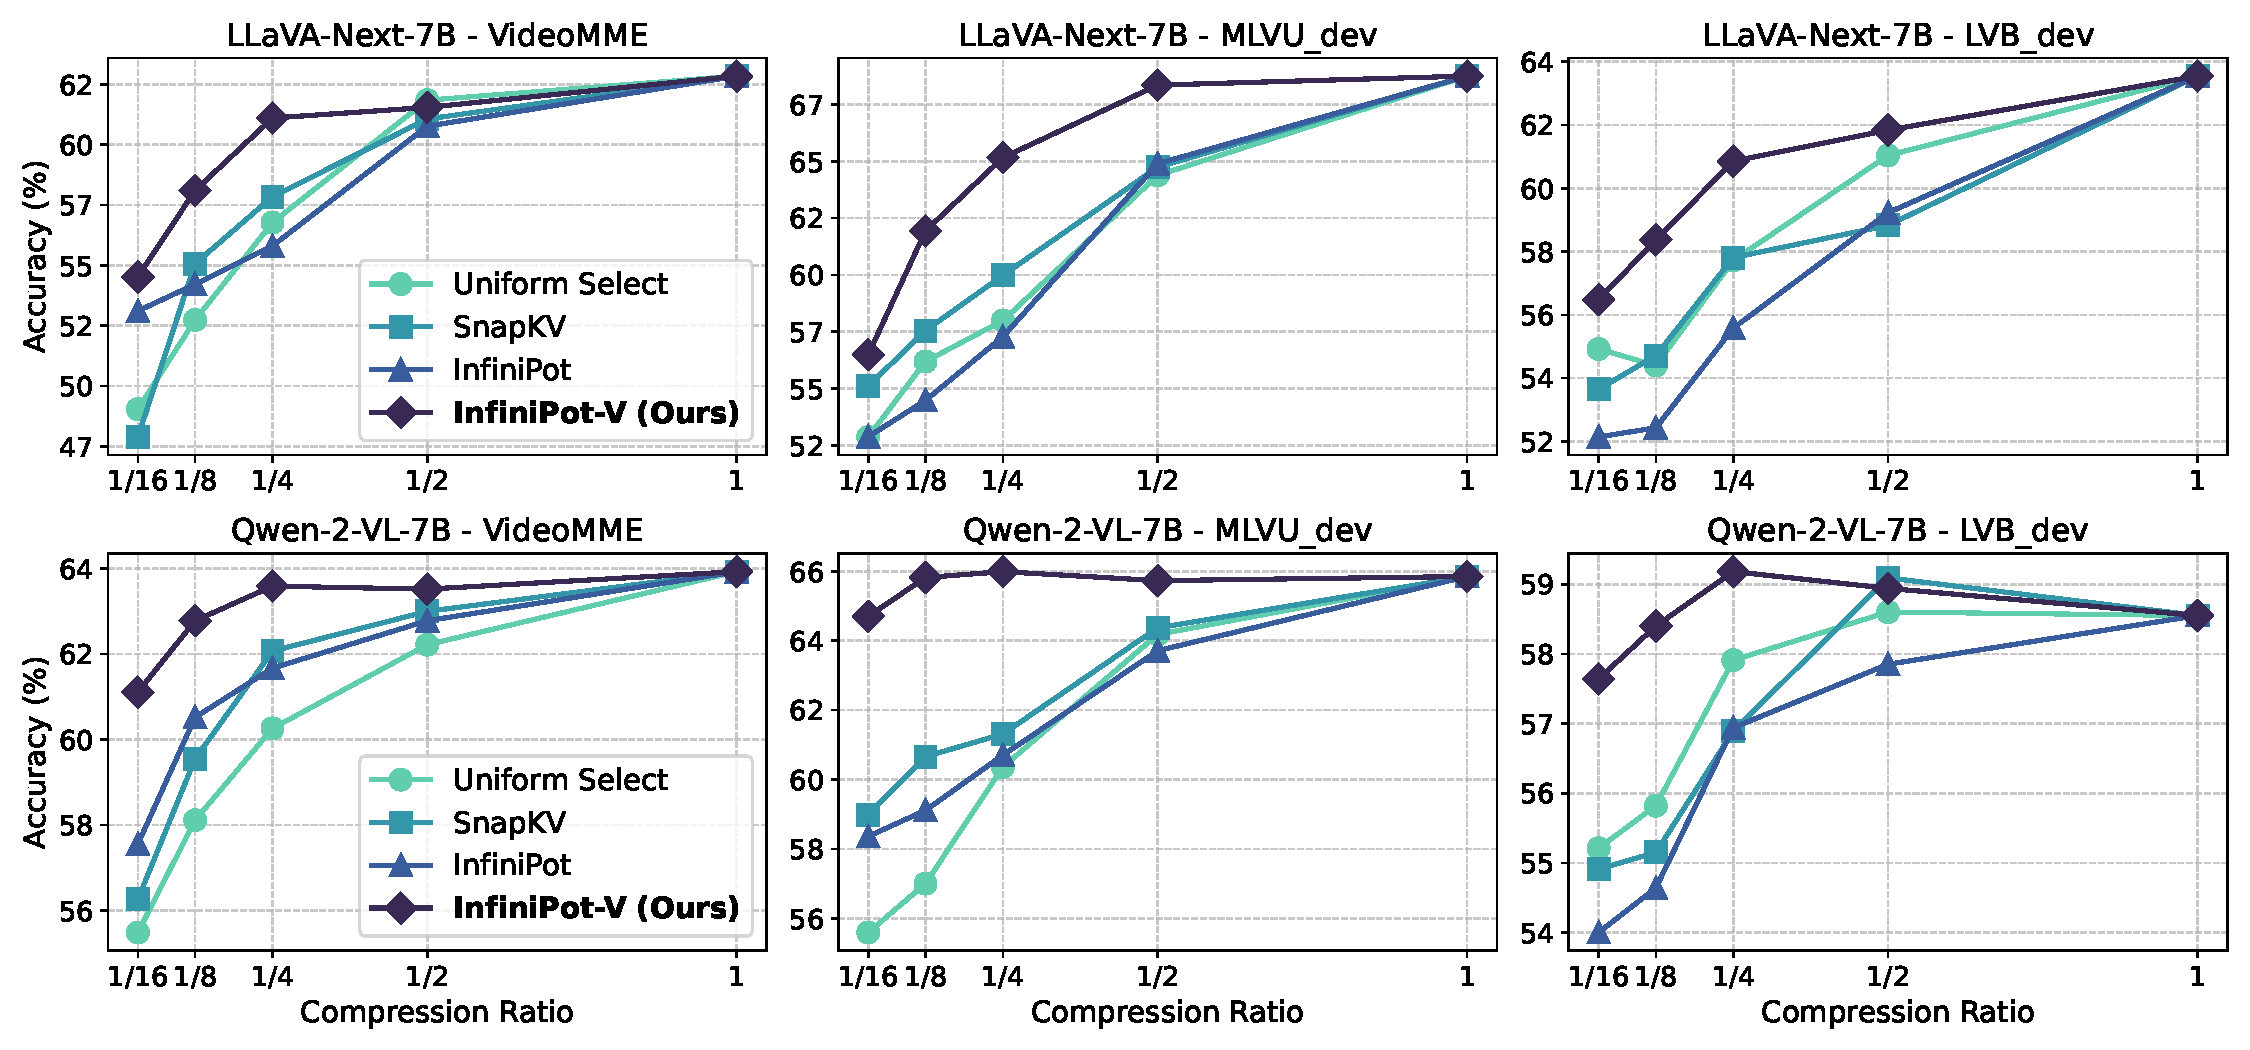
\includegraphics[width=1\columnwidth]{Figures/fig4_ver2.pdf}}
% \vspace{-.1in}
\caption{Resultados de evaluación de métodos de KV cache Compression (KVC) con tareas offline de long video understanding bajo el marco de Continual KV Cache Compression (CKV). Rendimiento en cuatro razones de compresión (1/16, 1/8, 1/4, 1/2) para \texttt{LLaVA-Next-7B} (fila superior) y \texttt{Qwen-2-VL-7B} (fila inferior) en las tareas VideoMME, MLVU$_\text{dev}$ y LongVideoBench$_\text{dev}$ (LVB$_\text{dev}$). Los resultados completos de evaluación se muestran en la Tabla~\ref{tab:full_table}.}\label{fig:kvc}
\vspace{-.1in}
\end{figure}

\subsection{Configuración experimental}

\paragraph{Benchmarks.}
Evaluamos nuestro InfiniPot-V tanto en tareas de offline video understanding (OVU) como de streaming video understanding (SVU). 
Para OVU, utilizamos benchmarks representativos de long video understanding basados en múltiple opción (desde 3 minutos hasta más de 2 horas): VideoMME~\cite{fu2024videomme}, MLVU~\cite{MLVU}, LongVideoBench (LVB)~\cite{wu2024longvideobench} y EgoSchema~\cite{mangalam2023egoschema}. 

Para SVU, empleamos el benchmark de streaming video QA RVS-Ego/Movie~\cite{zhang2024flashvstream}, que presenta preguntas abiertas emparejadas con timestamps, y evaluamos las respuestas usando \texttt{GPT-3.5-turbo-0125} siguiendo~\cite{zhang2024flashvstream,Shangzhe2025streaming}. 
Además extendemos la evaluación de SVU basada en múltiple opción con OVO-Bench~\cite{li2025ovobenchfarvideollmsrealworld} y StreamingBench~\cite{lin2024streaming}. 
OVO-Bench evalúa razonamiento temporal bajo tres escenarios---trazado retrospectivo, percepción visual en tiempo real y respuesta activa hacia adelante---mientras que StreamingBench evalúa comprensión visual en tiempo real de videos en streaming.

\paragraph{Modelos.}
Aplicamos nuestro método sobre cuatro MLLMs de estado del arte capaces de long-video understanding: Qwen-2-VL~\cite{Qwen2VL}, Qwen-2.5-VL~\cite{qwen2.5}, LLaVA-OV-7B~\cite{li2024llava} y LLaVA-Next-Video~\cite{zhang2024llavanext-video}. Los detalles sobre las configuraciones de muestreo del video de entrada y del benchmark se proporcionan en el Apéndice.~\ref{appn:exp}.

\subsection{Resultados de evaluación}
\paragraph{Offline Video Understanding. } 
Para evaluar la capacidad absoluta de compresión de nuestro método, evaluamos InfiniPot-V tanto con MLLMs comerciales (GPT-4V~\cite{openai2023gpt4v}, GPT-4o~\cite{openai2023gpt4o}) como con modelos públicos de estado del arte diseñados para offline video understanding, incluyendo LLaVA-OV~\cite{li2024llava} y LongVU~\cite{shen2024longvu}. A diferencia de estos modelos especializados y completamente entrenados, InfiniPot-V es un framework plug-in sin entrenamiento, compatible con MLLMs de distintas escalas, que permite alto rendimiento bajo presupuestos de memoria fijos.
Como se muestra en la Tab.~\ref{tab:open-source}, InfiniPot-V reduce el uso de memoria a solo 25\% (6K tokens) para LLaVA-Next (originalmente 25K tokens) y a 12.5\% para la serie Qwen-VL (6K frente a 50K), con una pérdida mínima de rendimiento. Notablemente, logra una exactitud comparable o mejor que LongVU a escala 7B y lo supera significativamente en 3B, demostrando tanto eficiencia como escalabilidad.

\paragraph{Comparación con IVC bajo restricciones de memoria.}
Para evaluar métodos IVC recientes independientes de la consulta bajo CKV restringido en memoria, adoptamos una configuración unificada sobre VideoMME y MLVU: token temporal merging (TTC) de DyCoke~\cite{tao2024dycokedynamiccompressiontokens} y spatial token compression (STC) de LongVU~\cite{shen2024longvu} se aplican para comprimir vision tokens hasta ajustarse al presupuesto de memoria objetivo $|M|$, mientras la KV cache se gestiona usando sliding window attention (SWA)~\cite{Beltagy2020Longformer}. Cuando operan bajo estas restricciones, estos métodos IVC sufren una degradación notable de exactitud. En contraste, InfiniPot-V realiza compresión de KV cache usando TaR y VaN, aprovechando representaciones key-value expresivas para lograr una exactitud promedio superior bajo un presupuesto de memoria de 6K, correspondiente a una tasa de compresión sin pérdida del 88\%.

\paragraph{Comparación con KVC bajo restricciones de memoria.}
La Fig.\ref{fig:kvc} evalúa métodos KVC dentro de nuestro marco CKV bajo memoria restringida en tareas de offline video understanding. Las razones de compresión (1/16, 1/8, 1/4, 1/2) se definen según la capacidad máxima de frames de cada modelo (por ejemplo, 128 frames para LLaVA-Next y 768 para Qwen-2-VL). Nuestro InfiniPot-V supera consistentemente a todos los métodos baseline (Uniform Select, SnapKV, InfiniPot) en todas las tareas tanto para LLaVA-Next-7B como para Qwen-2-VL-7B, demostrando un rendimiento superior de video understanding. Bajo restricciones CKV---donde no se dispone de la consulta real---los métodos dependientes de la consulta como SnapKV\cite{li2024snapkv} se degradan significativamente. En contraste, InfiniPot-V mantiene una exactitud sólida incluso con razones altas de compresión (por ejemplo, 1/16), gracias a su selección independiente de la consulta mediante TaR y VaN.

\begin{table}[t]
    \small
  \centering
  \begin{tabular}{l c c c c c c c c c}
    \toprule
    & \multicolumn{2}{c}{\textbf{RVS-Ego}} & \multicolumn{2}{c}{\textbf{RVS-Movie}} & \textbf{Execution Time }
    & \multicolumn{2}{c}{\textbf{Total Memory Usage}} \\ 
    \cmidrule(lr){2-3} \cmidrule(lr){4-5} \cmidrule(lr){6-6} \cmidrule(lr){7-8}
       \textbf{LLaVA-OV-7B} & \textbf{Acc} & \textbf{Score} & \textbf{Acc} & \textbf{Score} & \textbf{Video Enc. (msec/Frame)} 
      & \textbf{GPU} & \textbf{CPU} \\
    \midrule
    ReKV                   & 60.1 & 3.9 & 53.4 & 3.8  &  285.7  & 37.5 GB & + 18.8GB/h \\ \midrule
    ReKV w/o off.       & 55.8 & 3.3 & 50.8 & 3.4  & 74.6  & 27.2 GB     & 0          \\
    InfiniPot-V                   & \textbf{57.9} & \textbf{3.5} & \textbf{51.4} & \textbf{3.5}  & 76.3  & 27.8 GB     & 0          \\
    \bottomrule
  \end{tabular}
  \vspace{2mm}
  \caption{Comparación en benchmark de streaming frente a un método de control de caché KV basado en offloading. (ReKV) Video Enc. muestra el tiempo de ejecución por frame, GPU indica el uso pico de memoria y CPU denota el tamaño de la video KV-Cache descargada a CPU por hora. Resultados basados en un video de 1 hora procesado con una tasa de muestreo de 0.5 fps en modo streaming. \texttt{Se usa LLaVA-OV-7B.}}
  \vspace{-.2in}
  \label{tab:rvs_ego_performance}
\end{table}

\begin{table}[t]
\small
\centering
\begin{tabular}{l c c c c c c c}
\toprule
\textbf{Qwen-2.5-VL} & \textbf{Scale}
& \textbf{OVO-BW} & \textbf{OVO-Real} & \textbf{OVO-FW} 
& \textbf{OVO-Avg} & \textbf{StreamingBench} \\
\midrule
Uniform Select & 7B & 44.5 & 61.1 & 47.8 & 51.7 & 75.2 \\
InfiniPot-V & 7B & 47.6 & 65.9 & 47.9 & \textbf{53.6} & \textbf{76.4} \\
\bottomrule
\end{tabular}
\vspace{.1in}
\caption{Comparison on OVO-Bench (BW: Backward, Real: Realtime, FW: Forward) and StreamingBench (Real-time visual understanding) using \texttt{Qwen-2.5-VL-7B} under 4K memory budget.}
\label{tab:ovo_results}
\vspace{-.2in}
\end{table}


\paragraph{Streaming Video Understanding.}
Primero evaluamos InfiniPot-V en streaming video understanding (SVU) usando dos benchmarks de StreamingVQA, RVS-Ego y RVS-Movie, con LLaVA-OV-7B.
Como baseline, comparamos contra ReKV~\cite{Shangzhe2025streaming}, un método SVU de estado del arte, bajo dos configuraciones: 
(1) CPU--GPU con offloading a CPU, que permite volcar la KV cache a memoria CPU, y 
(2) CPU--GPU sin offloading, simulando dispositivos de memoria compartida donde la memoria CPU no está disponible o ya está ocupada~\cite{Karumbunathan2022JetsonAGXOrin}. 
La Tab.~\ref{tab:rvs_ego_performance} reporta exactitud SVU, tiempo de compresión y uso de memoria. 
Mientras que el offloading a CPU permite a ReKV retener la KV cache completa, introduce una sobrecarga sustancial de transferencia; sin offloading, ReKV sufre una degradación severa de exactitud debido a la memoria local limitada. 
En contraste, InfiniPot-V opera completamente dentro de la memoria GPU, elimina la latencia de offloading y alcanza mayor exactitud, lo que lo convierte en una solución práctica para sistemas con memoria restringida.

Para evaluar aún más la exactitud en escenarios de streaming, extendemos el análisis a dos benchmarks adicionales: OVO-Bench~\cite{li2025ovobenchfarvideollmsrealworld} y StreamingBench~\cite{lin2024streaming}, como se resume en la Tab.~\ref{tab:ovo_results}. 
En comparación con el baseline de selección uniforme de tokens, InfiniPot-V muestra mejoras consistentes en todas las métricas, mejorando notablemente el recall de información visual pasada en la tarea OVO-BW (backward) (44.5 $\rightarrow$ 47.6) y logrando mayor exactitud de comprensión en tiempo real en OVO-Real (Realtime) (61.1 $\rightarrow$ 65.9) y en la puntuación de StreamingBench (75.2 $\rightarrow$ 76.4), demostrando la efectividad de nuestra compresión TaR--VaN para eliminar redundancia temporal mientras preserva semántica espacialmente saliente, y mostrando su capacidad bajo escenarios SVU exigentes.

\subsection{Estudio de ablación}
\begin{table}[t]
\small
  \centering
  \begin{tabular}{l c c c c c c c c}
    \toprule
    \textbf{MLVU}$_\text{dev} $& \multicolumn{2}{c}{\textbf{Holistic Reasoning}} 
    & \multicolumn{3}{c}{\textbf{Single Detail}} 
    & \multicolumn{2}{c}{\textbf{Multi Detail}} \\
    \cmidrule(lr){2-3} \cmidrule(lr){4-6} \cmidrule(lr){7-8}
    \textbf{Ablation Study} 
      & \textbf{Topic}  & \textbf{Anomaly} 
      & \textbf{Plot}   & \textbf{Needle} 
      & \textbf{Ego}    & \textbf{AO} 
      & \textbf{AC}     & \textbf{Avg} \\
    \midrule
    Full KV           & 85.2 & 67.5 & 72.7 & 83.9 & 65.1 & 54.1 & 32.5 & 65.9 \\ \midrule
    Uniform Select    & 83.7 & 66.5 & 67.9 & 76.1 & 58.5 & 51.0 & 27.2 & 61.5 \\ \midrule
    TaR Reverse       & 79.0 & 64.5 & 56.9 & 65.6 & 55.1 & 45.2 & 21.8 & 55.5 \\
    TaR Frame         & 82.9 & 66.0 & 67.0 & 78.9 & 63.6 & 51.0 & 31.1 & 62.9 \\
    TaR               & 85.9 & 66.5 & 71.8 & 78.0 & 62.2 & 51.7 & 35.4 & \textbf{64.5} \\ \midrule
    VaN Reverse       & 78.3 & 66.5 & 56.2 & 66.8 & 53.4 & 46.3 & 17.5 & 55.0 \\ 
    VaN               & 84.4 & 68.0 & 68.6 & 76.6 & 61.9 & 52.5 & 29.1 & 63.0  \\ 
    VaN + Pool        & 85.2 & 68.0 & 71.4 & 77.5 & 63.1 & 52.1 & 31.5 & \textbf{64.1} \\ \midrule
    % TaP + VaN         & 84.0 & 67.0 & 71.1 & 79.2 & 61.9 & 51.7 & 31.6 & 63.8 \\
    % TaP + 1D-VaN      & 84.4 & 67.0 & 71.2 & \textbf{80.9} & 62.1 & 52.1 & 33.0 & 64.4 \\
    % TaP + 2D-VaN      & 85.9 & 67.5 & \textbf{72.9} & 79.4 & 62.2 & 52.9 & \textbf{35.9} & 65.3 \\ 
    TaR + VaN + Pool   & 86.3 & 68.0 & 72.7 & 80.3 & 63.9 & 54.1 & 35.4 & \textbf{65.8} \\
    \bottomrule
    \vspace{1mm}
  \end{tabular}
  \caption{Estudio de ablación de TaR, VaN y su combinación. Experimentos realizados en MLVU usando \texttt{Qwen-2-VL-7B} con un presupuesto de memoria de 6K.}
    \vspace{-.2in}
\label{tab:ablate}
\end{table}
 


La Tab.~\ref{tab:ablate} valida nuestras decisiones de diseño para TaR y VaN. Las estrategias invertidas (TaR Reverse y VaN Reverse) degradan significativamente el rendimiento al descartar tokens distintivos o semánticamente importantes. Dentro de TaR, la similitud por patch demuestra ser más efectiva que la similitud a nivel frame (64.5 vs. 62.9). VaN por sí solo supera al baseline, y su rendimiento mejora aún más con adaptive pooling (64.1 vs. 63.0). Combinar TaR y VaN produce la mayor exactitud, superando significativamente al baseline. Exploraciones adicionales de integración se discuten en el Apéndice.~\ref{appn:hyper_parameter}.

\begin{table}[t]
\small
\centering
\begin{tabular}{l c c c c c c}
\toprule
\textbf{Method} & \textbf{Length} & \textbf{Context} &
\textbf{VRAM} & \textbf{FPS} & \textbf{Throughput} & \textbf{Power} \\
 & \textbf{(sec)} & \textbf{Length} &
\textbf{(GB) ↓} & \textbf{(frame/sec) ↑} & \textbf{(tok/sec) ↑} & \textbf{(J) ↓} \\
\midrule
Full KV & 100 & 18K & 13.8 & 6.2 & 5.0 & 1.6 \\
InfiniPot-V    &     &     & 9.2 (1.5$\times$) & 6.4 (1.0$\times$) & 9.2 (1.8$\times$) & 1.2 (1.4$\times$) \\ \midrule
Full KV & 300 & 54K & 26.6 & 5.0 & 2.0 & 4.7 \\
InfiniPot-V    &     &     & 10.1 (2.6$\times$) & 6.4 (1.3$\times$) & 9.2 (4.6$\times$) & 2.4 (2.0$\times$) \\ \midrule
Full KV & 500 & 90K & 39.0 & 4.1 & 1.2 & 7.5 \\
InfiniPot-V    &     &     & 10.7 (3.6$\times$) & 6.3 (1.5$\times$) & 9.1 (7.3$\times$) & 3.7 (2.0$\times$) \\ \midrule
Full KV & 600 & 108K & OOM & OOM & OOM & OOM \\
InfiniPot-V    &      &      & 11.3 & 6.4 & 9.2 & 4.3 \\
\bottomrule
\end{tabular}
\vspace{.1in}
\caption{Resultados de rendimiento del procesamiento de streaming video en NVIDIA Jetson AGX Orin. Muestras de video en streaming de 10 minutos (FPS 0.2--1) procesadas con Qwen-2.5-VL-3B, midiendo memoria, FPS (frames procesados por segundo), throughput y consumo de energía.}
\label{tab:jetson}
\vspace{-.2in}
\end{table}


\subsection{Resultados de despliegue en dispositivos edge}
\label{sec:deployment}

Evaluamos nuestro marco CKV---que combina compresión continua de KV con puntuación TaR y VaN---en NVIDIA Jetson AGX Orin~\cite{Karumbunathan2022JetsonAGXOrin} usando \texttt{Qwen-2.5-VL-3B} y videos de 10 minutos de StreamingBench~\cite{lin2024streaming} (0.2--1 FPS). Como se muestra en la Tab.~\ref{tab:jetson}, nuestro método logra una eficiencia consistente en todas las métricas. La memoria pico permanece casi constante (9.2--10.7\,GB) mientras que Full KV crece linealmente (13.8→39.0\,GB), logrando una reducción de 3.6$\times$ a los 500 segundos de video en streaming. La velocidad de Prefill, medida en FPS (frames procesados por segundo durante el prefill), se mantiene estable en 6.3--6.4\,FPS, mientras que Full KV cae a 4.1\,FPS. El throughput de generación también aumenta hasta 7.3$\times$ (1.2→9.1\,tok/sec) bajo un presupuesto fijo de memoria. El consumo de energía escala proporcionalmente con el cómputo, mejorando la eficiencia energética en casi 2$\times$ (7.5→3.7\,J). Notablemente, CKV permite inferencia continua en flujos de 600 segundos donde Full KV falla con OOM, confirmando su practicidad para razonamiento multimodal en tiempo real sobre dispositivos edge con memoria restringida.
